\chapter{Introduction}
\label{introduction}

\section{Infandango}
Infandango is an automated web-based marking system for student submitted programming exercises, currently only for the Java language. A student can view the list of warm-up, optional and core exercises and choose to submit a file for one of them. Jester is the testing daemon for Infandango which compiles and runs code inside a sandbox for security purposes. Between the web frontend and Jester there is a PostgresSQL database which stores the source code of each submission and the score information for each marked submission.

Each question has a label: {\bf warmup} questions are simple questions which can be skipped if the user feels confident, {\bf core} questions are questions which the user is highly encouraged to try and may affect the end coursework mark, and {\bf optional} questions are provided for particularly interested students.

\subsection{Current feedback}
The primary source of feedback in Infandango is displayed in Figure \ref{fig:currentfeedback}. Each submission is marked with a set of JUnit tests and the fraction of these tests which are correct is displayed. This fraction is converted into a percentage and displayed on a red (0 - 40\%), orange (40\%-70\%) or green (70\%-100\%) background.
More general feedback is also available which displays similar information but the results are displayed by week rather than by question. 

\begin{figure}[h!]
\centering
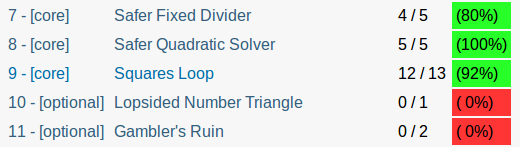
\includegraphics[width=0.8\textwidth]{images/currentfeedback.png}
\caption{This is a cropped screenshot of what is displayed to the user for a given week in the current Infandango system}
\label{fig:currentfeedback}
\end{figure}

\subsection{Current Use}
The system has been used with the first year Java programming course at the University of Edinburgh for a few years. The database information for these years has been kept and retains all the information about submissions: marks, submission time, number of resubmissions. The database for one year has been anonymised and made available for use in this project if necessary. Only one year is available because the questions have changed since previous years and therefore the data would be inconsistent with the current questions.

\section{Project Goals}
The general goal of this project was to improve the feedback for the open source web-based marking system, Infandango\cite{infandango_note}. In order to achieve this, a list of objectives was created to facilitate the research, design and implementation of a suitable modification to the system:

\begin{enumerate}
\item Research and investigate current systems for providing automatic feedback to students. Examples where this feedback pertains to code are of particular interest.
\item Through evaluation of both the literature and the system choose an appropriate approach for providing feedback.
\item Implement the approach and then, when it is functional, integrate with the Infandango system.
\item Perform user evaluation of the completed work to determine any impact it has on the learning of the student
\end{enumerate}

Most of this report will be discussing how these objectives have been realised and the extent to which they have been completed will be discussed in Chapter \ref{conclusion}.
